\subsection{Perturbacijos}\label{sec:literature:perturbations}

Perturbacijos -- tai pagrindinis obfuskacijos metodas \gls{ae} kūrimui.
Perturbacijų tikslas yra pakeisti kenkėjiškos programos veikimą išsaugant
originalų funkcionalumą. Perturbacijos gali būti sudėtingos ir apimti visą
programą (pvz., visos programos užšifravimas ir pridėjimas prie kitos
programos), semantinės (pvz., tam tikrų mašininio kodo instrukcijų keitimas į
ekvivalentų rezultatą pasiekiančias) arba baitų lygio (pvz., nulinių baitų
pridėjimas programos gale) \cite{huGeneratingAdversarialMalware2017}. Perturbacijų parinkimas įeina į
\glsko{framework} apibrėžimą. Šiame poskyryje aptariamos mokslinėje
literatūroje minimos perturbacijos.
\subsubsection{Baitų lygio perturbacijos}\label{sec:literature:perturbations:byte}
Pačias paprasčiausias baitų lygio perturbacijas galima taikyti bet kokio formato failams, tačiau labiau prasmingos perturbacijos taikomos \gls{pe} formato failams. Išskiriamos šios pagrindinės baitų lygio perturbacijos:
\begin{itemize}
    \item \textbf{\textit{ARBE} (\textit{Append Random Bytes at the End})} \cite{fangEvadingMalwareEngines2019}. \gls{pe} formato failo gale pridedami atsitiktiniai baitai.
    \item \textbf{\textit{ARI} (\textit{Append Random Import})} \cite{fangEvadingMalwareEngines2019}. \gls{pe} formato failo \textit{ImportAddressTable} lentelėje pridedama atsitiktinai pavadinta biblioteka su atsitiktinai pavadinta funkcija.
    \item \textbf{\textit{ARS} (\textit{Append Randomly named Section})} \cite{fangEvadingMalwareEngines2019}. \gls{pe} formato failo \textit{SectionTable} lentelėje pridedamos atsitiktinės sekcijos (sekcijos ir jų tipai yra apibrėžti \gls{pe} formate).
    \item \textbf{\textit{RS} (\textit{Remove Signature})} \cite{fangEvadingMalwareEngines2019}. Sertifikato pašalinimas iš \gls{pe} formato failo \textit{CertificateTable} lentelės.
    \item \textbf{Naujas įeities taškas} \cite{andersonLearningEvadeStatic2018}. Prasidėjus programai, iškart peršokama nuo naujo įeities taško į originalųjį.
    \item \textbf{\textit{Header Fields}} \cite{demetrioAdversarialEXEmplesSurvey2021}. \gls{pe} formato failo \textit{PE Header} ir \textit{Optional Header} dalių specifinių laukų keitimas (pvz., sekcijos pavadinimo keitimas \cite{andersonLearningEvadeStatic2018}).
    \item \textbf{\textit{Partial DOS}} \cite{demetrioAdversarialEXEmplesSurvey2021}. \gls{pe} formato failo \textit{DOS Header} dalies pirmi 58 baitai po \textit{MZ} skaičiaus yra nenaudojami moderniose operacinėse sistemose, tad juos galima keisti.
    \item \textbf{\textit{Slack Space}} \cite{demetrioAdversarialEXEmplesSurvey2021}. Dėl \gls{pe} formato specifikos, kiekviena nauja sekcija turi prasidėti tam tikro skaičiaus, nurodyto \textit{PE Header} dalyje, kartotiniu nuo pradžios. Kompiliatoriai šį reikalavimą išpildo sekcijų gale pridėdami tiek nulinių baitų, kiek reikia teisingam sulygiavimui pasiekti. Būtent ši nulinių baitų erdvė gali būti keičiama be jokios įtakos originaliai programai.
    \item \textbf{\textit{Padding}} \cite{demetrioAdversarialEXEmplesSurvey2021}. Nulinių baitų pridėjimas failo gale.
    \item \textbf{\textit{Full DOS}} \cite{demetrioAdversarialEXEmplesSurvey2021}. Perturbacijos esmė tokia pat, kaip ir \textit{Partial DOS}, tik naudojami visi \textit{DOS} dalies baitai, išskyrus \textit{MZ} ir \textit{PE Offset} (\textit{Partial DOS} manipuliacijoms naudoja tik dalį tarp \textit{MZ} ir \textit{PE Offset}).
    \item \textbf{\textit{Extend}} \cite{demetrioAdversarialEXEmplesSurvey2021}. Pakeičiama \gls{pe} formato faile \textit{DOS} dalyje esanti \textit{PE Offset} reikšmė į didesnę\footnote{\label{footnote:structure}šios reikšmės padidinimas reiškia visos failo struktūros keitimą (\textit{DOS} dalis yra failo pradžioje). Būtina pakeisti visų sekcijų vietas nuo pradžios \angl{offset} jų metaduomenyse.}. Taip padidinama (išplečiama) visa \textit{DOS} dalis. Tolesnis perturbacijos principas yra toks pat, kaip ir \textit{Full DOS}.
    \item \textbf{\textit{Shift}} \cite{demetrioAdversarialEXEmplesSurvey2021}. \gls{pe} formato failuose kiekvienas sekcijos blokas prasideda su sekcijos vieta nuo pradžios \angl{offset}. Tarkime ši reikšmė yra $S$. Sekcijos kodas pradedamas vykdyti tik nuo adreso $P+S$, kur $P$ -- programos pradžios adresas. Vadinasi, padidinus\footnoteref{footnote:structure} $S$ per $n$, atsiranda $n$ baitų laisvos vietos iki sekcijos pradžios, kurią galima keisti be jokios įtakos programos veikimui.
\end{itemize}
\subsubsection{Semantinės perturbacijos}\label{sec:literature:perturbations:semantic}
Semantinių perturbacijų įgyvendinimas taip pat atliekamas baitų lygyje, tačiau šie pokyčiai turi aukštesnio lygio prasmę. Išskiriamos šios semantinės perturbacijos:
\begin{itemize}
    \item \textbf{Nereikalingų \hyperref[feature:dll]{DLL/API vardų} požymių pridėjimas} \cite{huGeneratingAdversarialMalware2017}. \gls{pe} formato faile \textit{ImportTable} lentelėje pridedami originalios programos nenaudojami \gls{dll}/\gls{api} vardai.
    \item \textbf{\textit{Binary Rewriting}} \cite{demetrioAdversarialEXEmplesSurvey2021}. Semantinis instrukcijų perrašymas. Pavyzdžiui, $A+B$ instrukcijos pakeitimas į $A-(-B)$.
\end{itemize}

\clearpage
\subsubsection{Kompleksinės perturbacijos}\label{sec:literature:perturbations:complex}
Kompleksinės perturbacijos yra pritaikomos tam tikriems tikslams. Obfuskacijos ir \glsplko{adversarial} tikslams literatūroje minimos šios kompleksinės perturbacijos:
\begin{itemize}
    \item \textbf{\textit{Obfusmal}} \cite{zhongMalFoxCamouflagedAdversarial2024}. Užšifruojama originalios programos kodo sekcija. Sukuriama ir originalios programos gale pridedama programa \textit{Shell.dll}, kurioje laikomas atšifravimo raktas, originalios programos kodo sekcijos adresas ir dydis. Be to, \textit{Shell.dll} geba atšifruoti originalios programos kodo sekciją ir jai perduoti kontrolę. \textit{Shell.dll} pridedama prie naudojamų \gls{dll}, o programos pradžios taškas nustatomas į \textit{Shell.dll} pradžios tašką. Iliustracija pateikiama \ref{fig:perturbations}-ame pav.
    \item \textbf{\textit{Stealmal}} \cite{zhongMalFoxCamouflagedAdversarial2024}. Visa originali programa užšifruojama ir pridedama prie programos \textit{Shell.exe} galo. \textit{Shell.exe} geba atšifruoti originalią programą ir perduoti jai kontrolę. Iliustracija pateikiama \ref{fig:perturbations}-ame pav.
    \item \textbf{\textit{Hollowmal}} \cite{zhongMalFoxCamouflagedAdversarial2024}. Užšifruojama visa originali programa. Ji pridedama prie kurios nors nekenksmingos programos galo. Prie šio junginio galo pridedama \textit{Hollow.dll} programa, kurios veikiamas panašus į \textit{Shell.exe} iš \textit{Stealmal}. Viso junginio pradžios taškas nustatomas į \textit{Hollowmal.dll} pradžios tašką. Iliustracija pateikiama \ref{fig:perturbations}-ame pav.
\end{itemize}

\begin{figure}[h]
    \begin{small}
        \begin{center}
            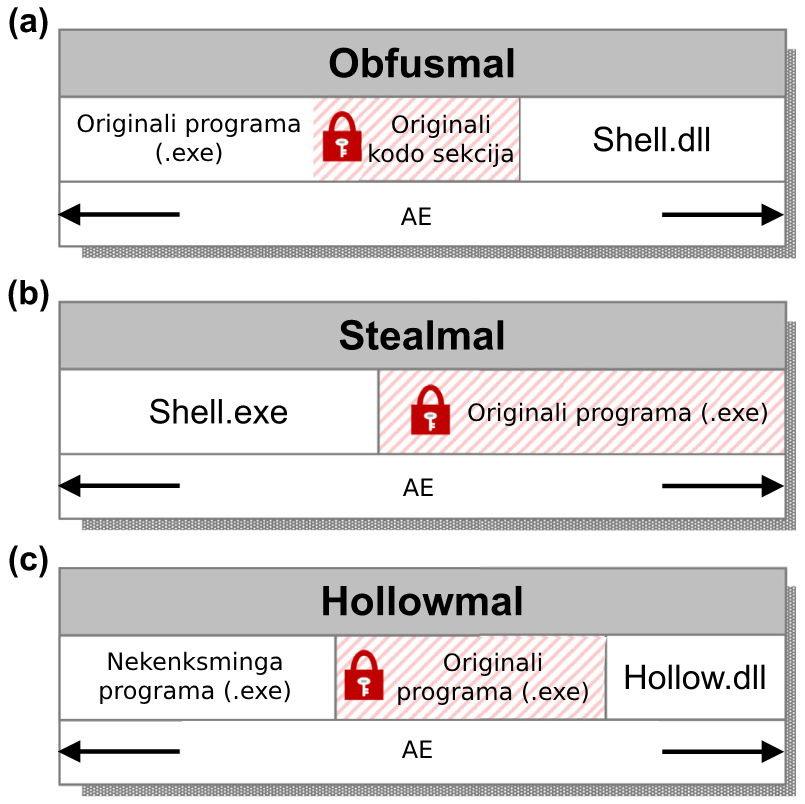
\includegraphics[width=0.4\textwidth]{images/complex-perturbations.png}
        \end{center}
        \caption{Obfusmal (a), Stealmal (b) ir Hollowmal (c) perturbacijų veikimo principų iliustracijos. Adaptuota iš \cite{zhongReinforcementLearningBased2022}}\label{fig:perturbations}
    \end{small}
\end{figure}
\clearpage